\documentclass{article}

\usepackage[a4paper,left=18mm,right=18mm,top=20mm,bottom=18mm]{geometry}
\usepackage[italian]{babel}

\usepackage{titling}
\usepackage{graphicx}
\usepackage{subcaption}
\usepackage{float}
\usepackage{hyperref}


\title{Documentation for Software engineering project}
\author{Nicolas Anselmi, David Guzman Piedrahita and Marco Vinciguerra}

\begin{document}
\maketitle
\section{Project Plan}
\subsection{Introduction}
Il progetto prevede lo sviluppo di una mobile app per gestire la prenotazione di 
un negozio di parruccheria. C'è la possibilità di avere due tipi di utente (anche in entrambe le modalità):
un cliente e un padrone di negozio. La novità di questo progetto consiste nel fatto che è un tipo di sistema P2P in cui un utente può essere contemporaneamente cliente
e (se vuole) gestore. Questo modello di business è fatto anche da Uber in cui un autista può essere sia cliente che autista.
\\Il target della clientela è market driven in quanto il core business dell'azienda si basa su percentuali delle transazioni.
Il cliente ha la possibilità di prenotare diversi    
tipi di acconciatura direttamente senza interfacciarsi /chiamare direttamente il proprietario
del negozio ma tramite l'applicazione.Ogni tipologia di taglio selezionabile ha una durata e in base al tipo dei macchinari e delle risorse che devono essere utilizzate 
e può consentire un orario customizzabile di prenotazione 
da parte del cliente. 
\\I membri del team sono: Nicolas Anselmi, David Guzman Piedrahita e Marco Vinciguerra.

\subsection{Process model}
Il life cycle del progetto è agile, in particolare la tecnica utilizzata è SCRUM con
sprint di 5 giorni in quanto il tempo necessario per lo sviluppo è breve. Inoltre viene utilizzato un triage per
gestire i compiti (MoSCoW).
\\Inoltre viene applicato un modello di prototipazione incrementale in cui ad ogni git viene aggiunto una funzionalità al sito e deve essere sempre disponibile
su Github una versione funzionante del progetto.
\\Per accelerare il processo di apprendimento viene applicato anche il processo di pair programming, 
pratica molto utilizzata nei metodi AGILE.
\\Per quanto riguarda i requirements si utilizza il Kano Model.
Il periodo di sviluppo parte poco prima di Natale. Ogni giorno verso le 9 30 del mattino 
c'è un daily scrum tenuto dallo scrum master in cui si discutono le problematiche riscontrate durante 
il giorno precedente e le possibili soluzioni a queste.

\subsection{Organization of the project}
Il progetto, dovuto alla sua natura, deve intefacciarsi sia con utenti  che usufruiscono del servizio di prenotazione, sia da utenti che mettono a disposizioni i loro servizi commerciali.
Il team di sviluppo è composto dai succitati integranti. Per portare a termine l'applicazione, ci sono dei knowledge-gap che dovranno essere colmati tramite la lettura di documentazione e
l'uso di risorse online: particolarmente nel caso del framework Flutter per il frontend development.

\subsection{Standards, guidelines, procedures}
Il principale linguaggio di programmazione del progetto sarà dart, quest'ultimo
viene esteso tramite flutter.
Si usano i coding standards di flutter per garantire la qualità.
\\Per gestire l'assegnazione e il corretto sviluppo si usa un template di Notion per gestire i compiti.
\\Gli IDE che vengono utilizzati sono: VSC e terminale con VIM.

\subsection{Management activities}
Ogni settimana viene fatto un report sui progressi in corso fatti dal team di sviluppo per avere un'idea sull'avanzamento del progetto.
\\Le modifiche critiche del progetto devono essere accettate dal padrone della cartella (Marco Vinciguerra), le altre possono essere fatte 
liberamente.
\\Questi report, insieme alle decisioni definite negli scrum meeting, rappresentano la principale strategia per valutare velocemente lo status del progetto, e, 
di conseguenza, sono utili a fare course-correction.
\\Difatti, è proprio in questo modo che è previsto bilanciare l’equilibrio tra requirements e l’impegno necessario per soddisfarli.  
\subsection{Risks}
Il rischio principale è di non consegnare in tempo il progetto o di non consegnare un progetto perfettamente funzionante.
\subsection{Staffing}
I membri del team sono: Nicolas Anselmi, David Guzman Piedrahita e Marco.
\\Per provare a vedere come funziona il mestiere il ruolo dello SCRUM master cambia a rotazione e si parte dalla settimana 
che inizia col 13 dicembre. Il primo SCRUM master sarà David, la settimana dopo Nicolas e quella dopo Marco Vinciguerra e così via...
\\Sono 3 studenti di ingegneria del terzo anno.

\subsection{Methods and techiniques}
Per gestire gli sprint è stato utilizzato un template di Notion in quanto ha la possibilità di schedulare i task in base alla scadenza e in base ad un ordine gerarchico.
\\Per gestire la fase di testing si usa il tool better flutter tests che fa lui il testing sul framework Flutter. Il test viene scritto automaticamente dal tool e quindi 
non si applica fin da principio.
\\Per quanto riguarda la specifica dei requisiti si utilizza lo standard IEEE 830.
\\Il design pattern utilizzato è il delegation pattern.
\\Si utilizza Flutlab.io per convertire il modello fatto con Figma in codice sorgente Flutter, questa è una strategia model driven.
\\Si prevede l'uso di una strategia COTS per la scelta di diversi moduli o, più precisamente, widget di Flutter, che consentono di implementare velocemente
elementi UI classici, senza scrivergli da zero.
\\Per quanto riguarda i test di Dart si utilizza Dart unit testing e si utilizza il TDD e per garantire la continuos integration si usa Travis CI che partirà ad ogni 
Git e ogni 24 ore.
\\Per i database non si fa nessun tipo di testing e si utilizza Firebase  per creare e gestire il database delle prenotazioni.
\\La gestione delle modifiche viene svolta tenendo in conto le considerazione del punto 5 e, soprattutto, il punto 13.
\subsection{Quality assurance}
Per garantire la qualità del prodotto viene utilizzato lo standard ISO 9001.

\subsection{Work packages}
Alcuni dei sottoprogetti (work package) che sono stati definiti a priori.
\\ In viste della natura agile del progetto, questi work-package saranno estesi e modificati o evoluti nelle diverse iterazioni del life-cycle:
\begin{itemize}
    \item Fase di design di schemi UML
    \item Imparare ad utilizzare Flutter e dart
    \item Implementare l'applicazione con un'interfaccia grafica (front-end)
    \item Implementare la domain logic (back-end)
    \item Uso di un database
    \item Fare il testing sul prodotto
    \item Fare testing usando l'applicazioni in telefoni reali (non simulator)
\end{itemize}

\subsection{Resources}
Gli obiettivi di prototipazione proposti dal progetto in questione richiedono solo l'uso di computer adatti alla programmazione nei suddetti linguaggi e framework.
Dopo diverse iterazioni di prototipazione è prevista la possibilità di usare dei cloud-server che ricevano e gestiscano le richieste degli utenti tramite i loro client/app. 

\subsection{Budget and schedule}
Il tempo preventivato per il progetto è di circa 55 ore a testa, quindi in totale saranno richieste 150 ore.
\\In particolare si prevede che saranno richieste 30 ore per fare la documentazione, 10 ore per imparare Flutter e dart, 10 ore per implementarla
e le restanti ore i database e il testing.
\subsection{Changes}
Col tempo potrebbero cambiare le richieste da parte del cliente durante la fase di validazione di ogni processo.
\\Al supporto delle attività di change management vengono utilizzati i due tool usati anche per altri aspetti del progetto, ovvero: 
\\Github, che in questo caso funge da piattaforma per accettare o rifiutare le modifiche version-oriented e per consentire di usare il forked develpment; 
\\e Notion che, non essendo un tool specifico per lo sviluppo, serve invece a gestire l’organizzazione delle tempistiche e dei sotto-progetti a un livello di astrazione più alto.
\\I contenuti di questi tool, e i diversi report dei punti precedenti, servono come guida per la compilazione di un eventuale configuration management plan che conterrà una management section e activities. I documenti generati come risultato del punto 5 sono particolarmente utili per la management section.

\subsection{Delivery}
Il project plan verrà consegnato entro il 27 dicembre 2021
\\La consegna verrà fatta 5 giorni prima dell'esame orale di gennaio.
\subsection{People Management and Team Organization}
\subsection{Software Quality}
\subsubsection{CMM}
Per quanto riguarda il CMM (Capaibility Maturity Model) esistono 5 livelli di maturità del software, essi sono:
\begin{itemize}
    \item Initial 
    \item Managed
    \item Defined
    \item Measurable
    \item Optimization
\end{itemize}
In questo progetto si punta ad utilizzare il terzo livello 3 (Defined) in cui ogni attività viene documentata
e standardadizzata per l'intera organizzazione del processo per il design, development e testing.

\subsubsection{ISO 9216}
Per quanto riguarda la product conformance si fa riferimento al seguente link: \url{https://www.geeksforgeeks.org/iso-iec-9126-in-software-engineering/}
\\Esso si basa sui 4 seguenti principi:
\begin{itemize}
    \item \textbf{Part 1: "Quality model"} 
    \item \textbf{Part 2: "External metrics"} 
    \item \textbf{Part 3: "Internal metrics"} 
    \item \textbf{Part 4: "Quality in use metrics"} 
\end{itemize}
Per chiarire meglio il concetto si fa riferimento al seguente grafico:
\\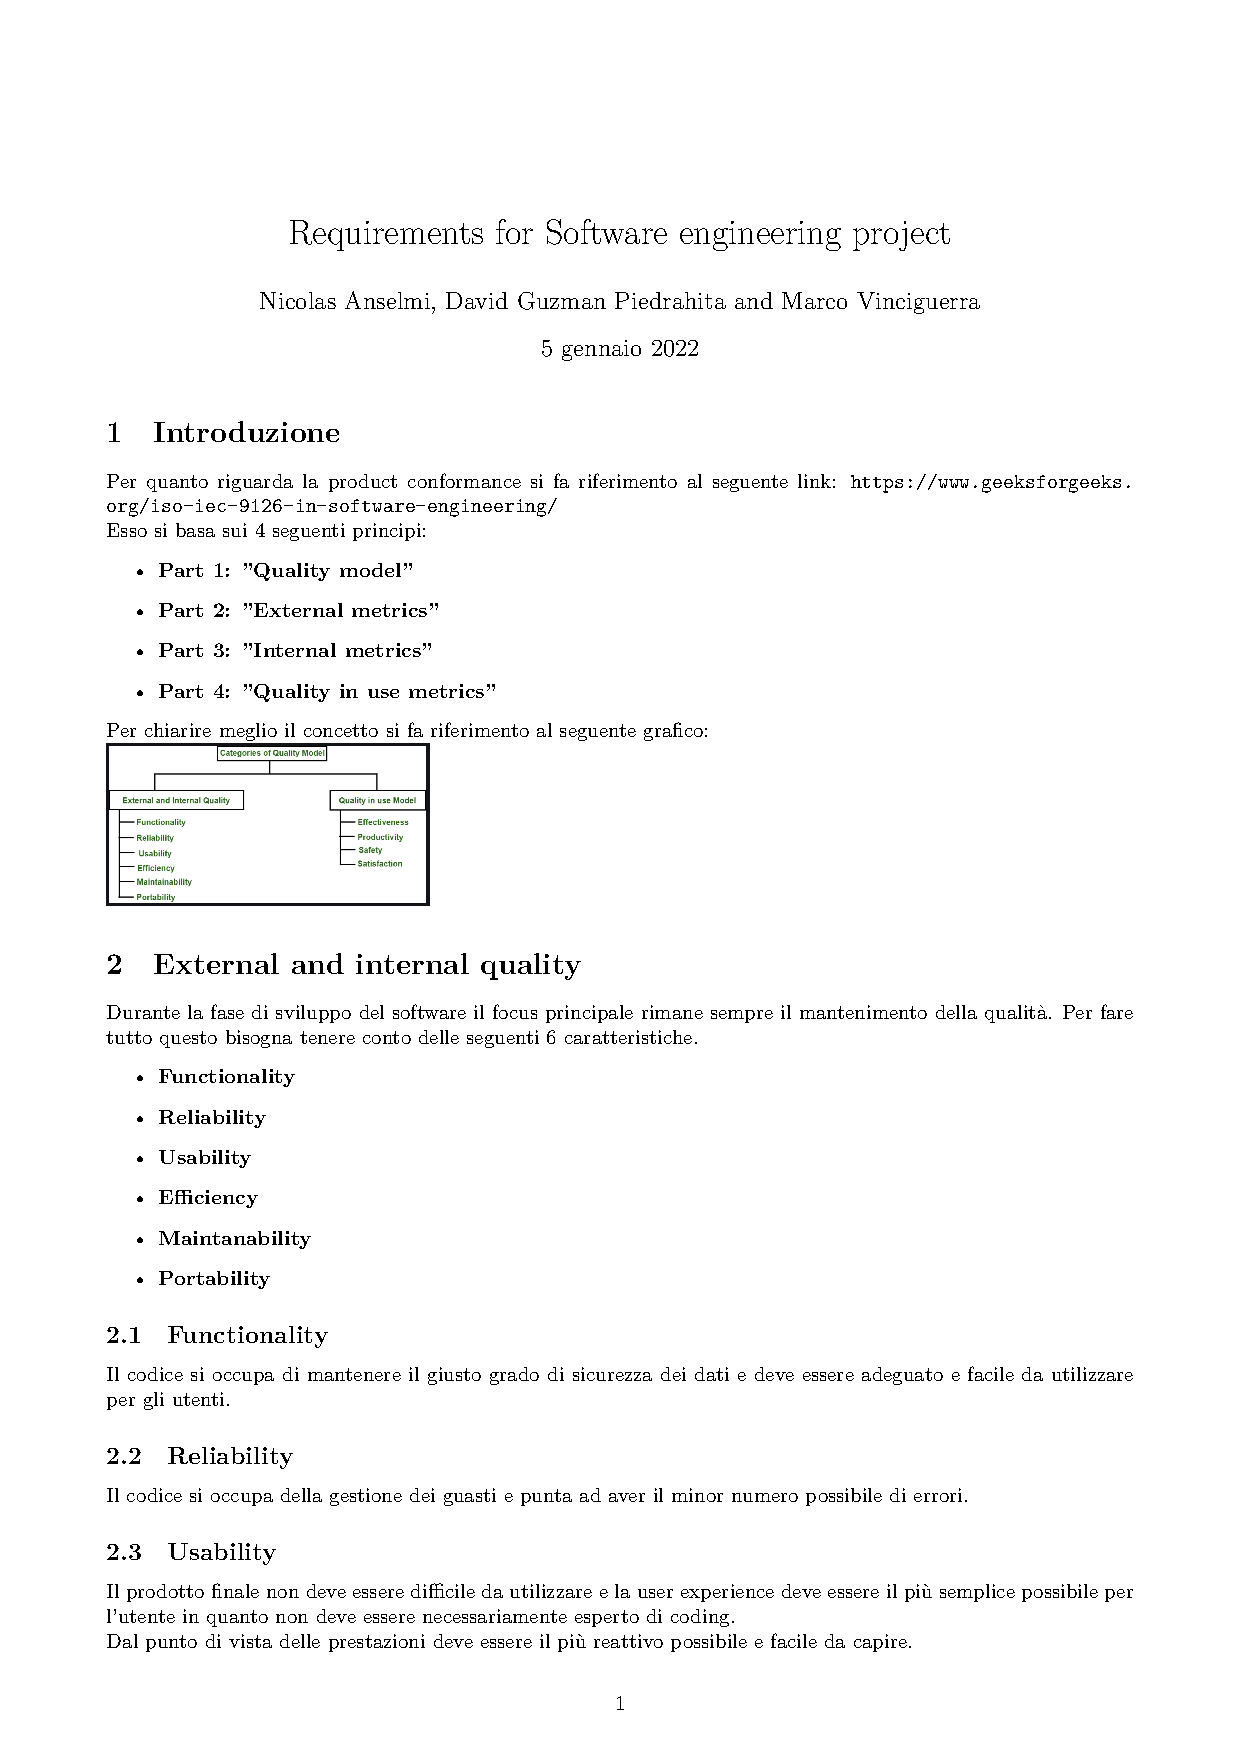
\includegraphics[scale = 0.25]{"Immagini/ISO9126.PNG"}
\section{External and internal quality}
Durante la fase di sviluppo del software il focus principale rimane sempre il mantenimento della qualità.
Per fare tutto questo bisogna tenere conto delle seguenti 6 caratteristiche.
\begin{itemize}
    \item \textbf{Functionality} 
    \item \textbf{Reliability} 
    \item \textbf{Usability} 
    \item \textbf{Efficiency} 
    \item \textbf{Maintanability} 
    \item \textbf{Portability} 
\end{itemize}

\subsection{Functionality}
Il codice si occupa di mantenere il giusto grado di sicurezza dei dati e deve essere adeguato e facile
da utilizzare per gli utenti.

\subsection{Reliability}
Il codice si occupa della gestione dei guasti e punta ad aver il minor numero possibile di errori.

\subsection{Usability}
Il prodotto finale non deve essere difficile da utilizzare e la user experience deve essere il più
semplice possibile per l'utente in quanto non deve essere necessariamente esperto di coding.
\\Dal punto di vista delle prestazioni deve essere il più reattivo possibile e facile da capire.

\subsection{Efficiency}
Si vuole creare il programma più efficiente possibile che utilizzi il minimo delle risorse del dispositivo
da cui si utilizza l'applicazione.

\subsection{Maintanability}
Il codice deve essere scritto nel modo più conforme alle regole di standard di programmazione per favorire
la leggibilità e la successiva manutenzione.

\subsection{Portability}
Il programma deve funziona su più piattaforme possibilil.

\section{Quality in use Model}
Si basa sulle seguenti 4 caratteristiche che si vuole soddisfare:
\begin{itemize}
    \item Effectiveness
    \item Productivity
    \item Safety
    \item Satisfaction 
\end{itemize}
\section{Requirement Engeneering-IEE830}
\subsection{Purpose} 
Questo documento segue la struttura proposta dallo standard IEEE 830 per la definizione dei requirements. Questi rappresenta uno dei criteri fondamentali per valutare l’adeguatezza dell’implementazione ottenuta nei diversi sprint e un punto di partenza per le seguenti fasi dello sviluppo dell’applicazione.
\subsection{Scope}
L’obiettivo centrale è costruire un’applicazione per la gestione di prenotazioni di tagli in saloni di bellezza, eventualmente estendibile ad altri servizi. 
\\In grandi linee, l’applicazione dovrebbe consentire di facilitare il processo della creazione di appuntamenti, evitando l’uso di chiamate, sostituendole con procedure online molto più veloci e friction-less. 
\\L’interfacciamento dell’utente con l’applicazione deve essere tale che, nonostante la più alta complessità inerente a una soluzione model-view-controller rispetto all’uso di semplici chiamate, l’utilizzatore percepisca un netto miglioramento rispetto al solito modo di fare e a prescindere delle loro conoscenze informatiche. 
\\Di conseguenza, l’applicazione non solo deve offrire la funzionalità centrale delle prenotazioni, ma in più deve farlo in un modo intuitivo. 

\subsection {Definitions, acronyms and abbreviations }
\subsection {References} 
\subsection {Overview} 
Dopo questa introduzione, il documento è composto da due ulteriori fasi: la parte 2, che da una descrizione globale dei requirements, e la parte 3, che elenca e classifica tutti i diversi requirements individuali, usando il modello Kano e Moscow.
\section {Overall description} 
\subsection {Product perspective} 
Non ci sono database o altre strutture informatiche preesistenti, in quanto il pubblico di destinazione è composto proprio da saloni di bellezza che gestiscono le loro prenotazioni in modo informale. La costruzione del software deve dunque partire da zero.
\\ Per la fase di elicitation sono state usate le strategie di open-ended interview, task analysis derivante anche da esperienze personali e natural language descriptions. 
\\ Le successive fasi di V and V e di negotiation saranno svolte dopo la generazione di un primo prototipo.
\subsection {Product functions} 
A continuazione sono elencati le funzionalità centrali, l’elenco dei requirements a una granularità più precisa sono disponibili nella parte 3.
\begin{itemize}
\item Possibilità di prenotare tagli e, eventualmente, altri servizi offerti dai saloni.
\item Possibilità di visualizzare le prenotazioni future e passate associate al salone in questione.
\item Possibilità di tener traccia dei clienti con degli appositi profili utente/cliente associati a informazioni rilevanti.
\item Disponibilità di visualizzare l’andamento dei ricavi risultanti dalle prenotazioni. 
\end{itemize}
\subsection {User characteristics} 
Come detto sopra, il prodotto deve essere costruito per soddisfare le esigenze di un pubblico di destinazione con conoscenze tecniche basilari (uso di smartphone e applicazioni user-friendly). 
\\L’UI dell’applicazione deve essere facile da usare da utenti ormai familiarizzatisi con altre applicazioni molto popolari (YouTube, Instagram…), di conseguenza il design-language deve essere coerente con quello al quale i potenziali utenti si sono ormai abituati, riducendo, di conseguenza, la learning-curve per usare il software.

\subsection {Constraints} 
Nella sua versione finale, l’applicazione dovrebbe essere utilizzabile sia da cliente che prenotano che da gestori di saloni di bellezza. 
\\I clienti dei saloni non devono avere accesso a informazioni del salone, come le prenotazioni di altri utenti, o i ricavi del salone. Dall’altro canto, i gestori non possono modificare certe informazioni dei profili degli utenti, ma possono modificare dati associati alle prenotazioni. 
\\Per il prototyping iniziale, si deve dare priorità alle funzionalità offerte ai gestori. L’implementazione delle prenotazioni remote fatte direttamente dagli utenti ha una priorità secondaria nelle prime fasi.
\subsection {Assumptions and dependencies}
\subsection {Requirements subsets} 
\section {Specific requirements}

\subsection{Kano model}
\subsubsection{Attractive:}
\begin{itemize}
    \item Possibilità di scegliere i diversi tipi di acconciature e in 
    base al tipo di acconciatura scegliere la durata della prenotazione 
\end{itemize}
\subsubsection{Must-be:}
\begin{itemize}
    \item Possibilità di registrarsi per la prima volta al sito da parte di un cliente.
    \item Utilizzo di un database per la gestione dei clienti. In alternativa si potrebbero utilizzare 
    variabili per gestire le prenotazioni.
    \item Creazione di un profilo base utente per le prenotazioni.
\end{itemize}

\subsubsection{One-Dimensional}
\begin{itemize}
    \item Che il sistema dellle prenotazioni non funzioni correttamente 
    e che si accavallino sulla stessa fascia oraria.
\end{itemize}

\subsubsection{indifferent:}
\begin{itemize}
    \item Troppa personalizzazione dell'utente (immagini + acconciature consigliate).
\end{itemize}
\subsubsection{Reverse:}

\subsubsection{Questionable:}
\begin{itemize}
    \item Possibilità di mettere recensioni da parte dell'utente.
\end{itemize}

\subsection{MoSCoW}

\subsection{Must haves}
\begin{itemize}
    \item Possibilità di scegliere i diversi tipi di acconciature e in 
    base al tipo di acconciatura scegliere la durata della prenotazione 
\end{itemize}

\subsection{Should haves}
\begin{itemize}
    \item Possibilità di registrarsi per la prima volta al sito da parte di un cliente.
    \item Utilizzo di un database per la gestione dei clienti. In alternativa si potrebbero utilizzare 
    variabili per gestire le prenotazioni.
    \item Creazione di un profilo base utente per le prenotazioni.
    \item Che il sistema dellle prenotazioni non funzioni correttamente 
    e che si accavallino sulla stessa fascia oraria.
\end{itemize}

\subsection{Could haves}
\begin{itemize}
    \item Possibilità di mettere recensioni da parte dell'utente.
\end{itemize}

\subsection{Won't haves}

\section{Software quality}
\subsection{Introduzione alla Taxonomy quality}
Questo file si occupa del descrivere i requisiti tassonomici di qualità del progetto.
\\Per quanto riguarda la definizione di McCall.
\\In particolare si vuole utiizare i seguenti driver/linee guifa per la produzione, revisione e
transizione  del codice.
\subsection{Product operation}
\begin{itemize}
    \item Correctness: se il sistema fa quello richiesto
    \item Reliability: se il sistema è abbastanza accurato
    \item Efficiency: se il sistema utilizza l'hardware efficientemente
    \item Integrity: se il sistema è sicuro
    \item Usability: se il sistema è utilizzabile
\end{itemize}
In particolare ci si sofferma sull'usability, correctness e reliability in quanto il 
prodotto deve funzionare il meglio possibile.

\subsection{Product revision}
\begin{itemize}
    \item Maintainability: se il sistema in caso di guasto è riparabile
    \item Testability: se il sistema è testabile 
    \item Felxibility: se il sistema è facilmente cambiabile
\end{itemize}
Il prodotto che si sta costruendo in questo caso tende a essere molto testabile in 
quanto i test per verificare la correttezza vengono creati ed eseguiti poco dopo la  creazione
delle classi.

\subsection{Product transition}
\begin{itemize}
    \item Portability: se il software è utilizzabile su altre piattaforme
    \item Reusability: se il software è riutilizzabile
    \item Interoperability: se il sistema è interfacciabile con altri sistemi
\end{itemize}
Il sistema tenderà a essere molto portabile in quanto è stato fatto con Flutter, il quale
tende ad essere molto scalabile.

\subsection{Qualità per il codice in Dart}
Per il codice in Dart è stato implementato il Dart Analyzer, che si ottiene modificando il file
$analysis_options.yaml$ e tramite il comando da terminale dart analyze si fa un test per 
vedere se le qualità prese in considerazione sono valide e rispettate.
\\La documentazione necessaria per informarsi su questo tipo di standard è stata presa
dal seguente link: \url{https://pub.dev/packages/analyzer}.
\\Alcuni tra i parametri presi in considerazione per garantire la qualità sono:

\begin{itemize}
    \item Maximum nesting level
    \item Ciclomatic complexity
    \item Number of parameters
    \item Source lines of code
\end{itemize}

Ecco un esempio di output di un test fatto con dart analyze:
\\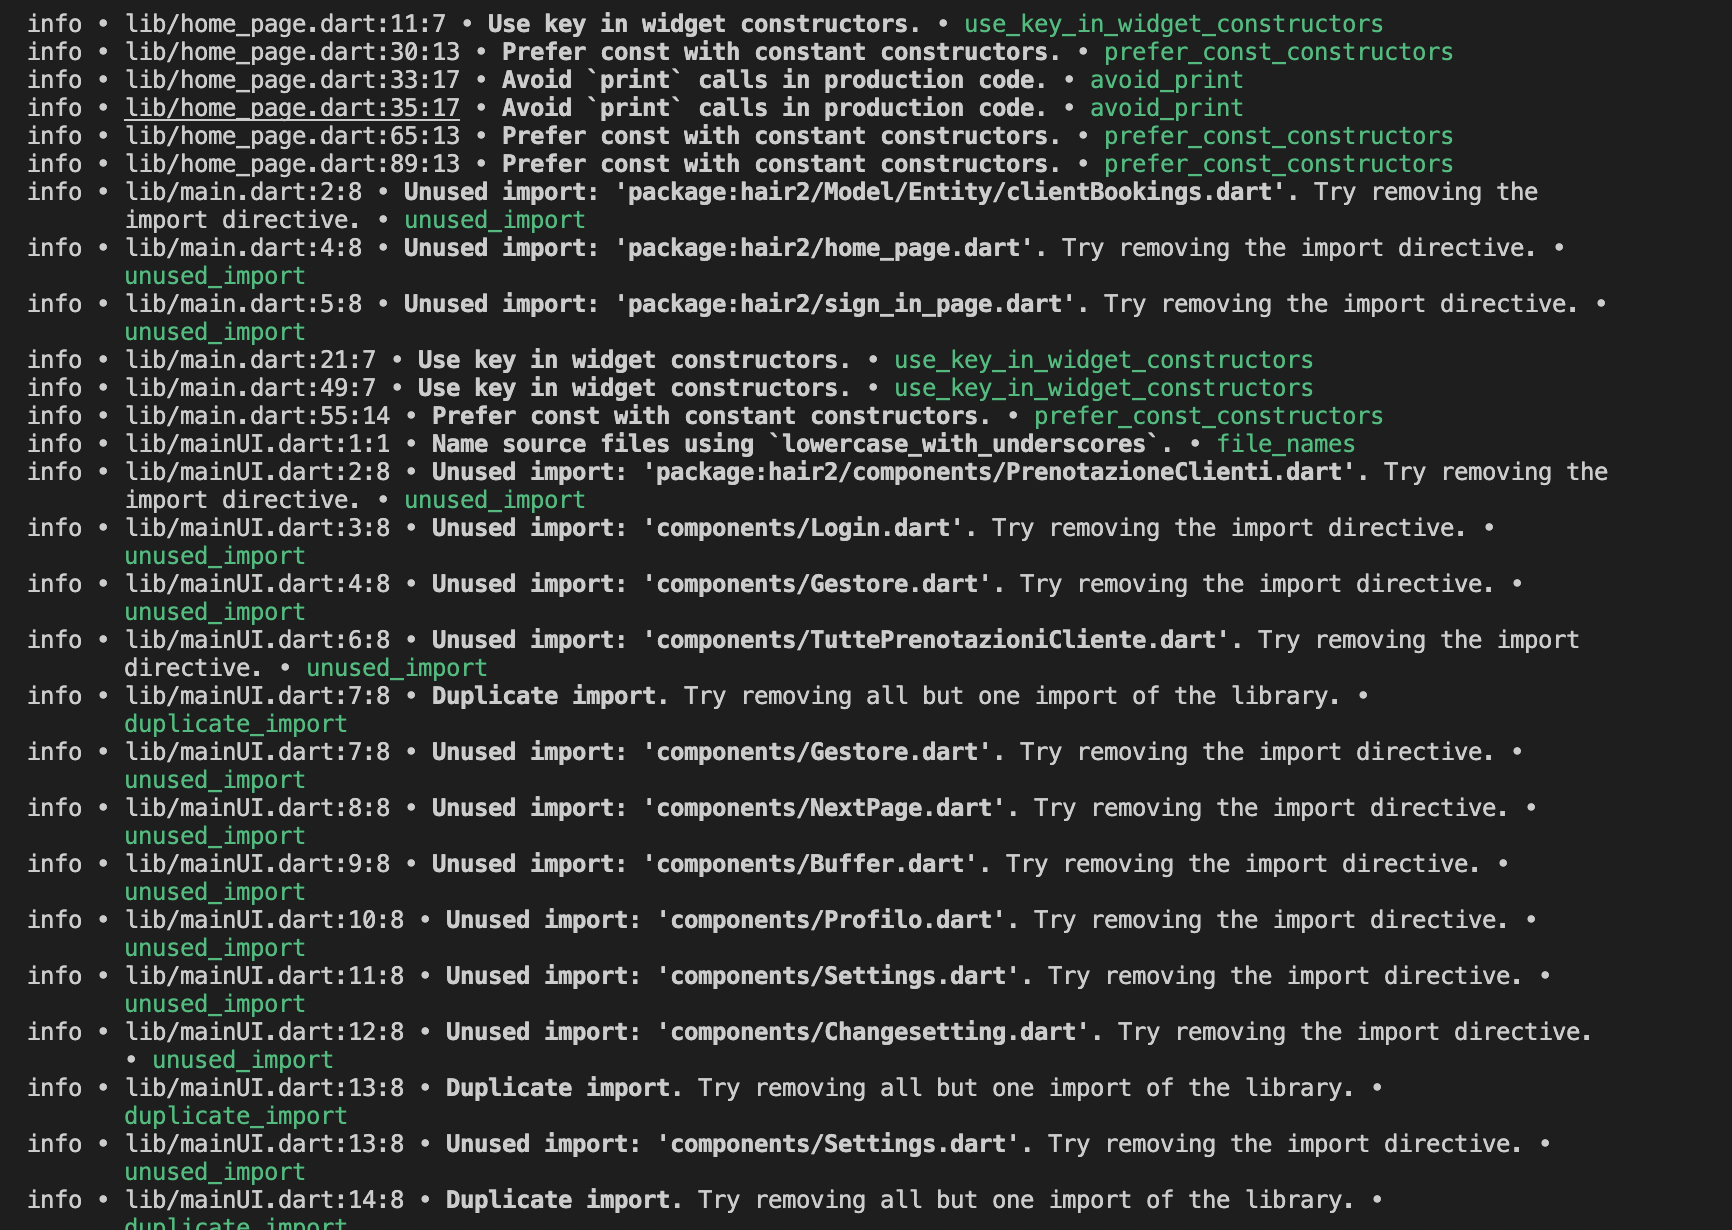
\includegraphics[scale = 0.5]{"Immagini/Dart_analyze.png"}
\\Questo era una run che indicava alcuni parametri da modificare per essere conformi ai
dart standards, in particolare si parla dell'utilizzo della keyword const.
\section{Software Architecture}
Per quanto riguarda i viewpoint sono stati rappresentati ad esempio due activity diagram per descrivere il progetto tramite due granularità e viewpoint differenti.
\subsection{Architecture design metod }
Per derivare una prima architettura funzionante partendo dai requirements specificati nell’apposito documento, si segue il criterio Generalized Model di Hofmeister et al. (2007).
\\Questo architecture design method è particolarmente utile per il progetto in questione, in quanto è strutturato utilizzando la terminologia e i ragionamenti di SCRUM, che è il life-cycle agile usato per l’applicazione e il suo sviluppo. 
\\In particolare, usa lo stesso concetto di backlog per elencare i diversi problemi che devono essere gestiti, e da esso è possibile scegliere gli elementi ritenuti più importanti in ogni particolare iterazione. 
\\Il backlog ha in input i requirements del progetto, con particolare attenzione ai requisiti di qualità; il contesto, che contiene idee aggiuntive sul come implementare un sistema che soddisfi i requisiti e, infine, i risultati della valutazione dell’architettura dell’iterazione precedente. 
\\Nel progetto verranno presi in considerazioni questi tre fattori per determinare le scelte di design. 
\\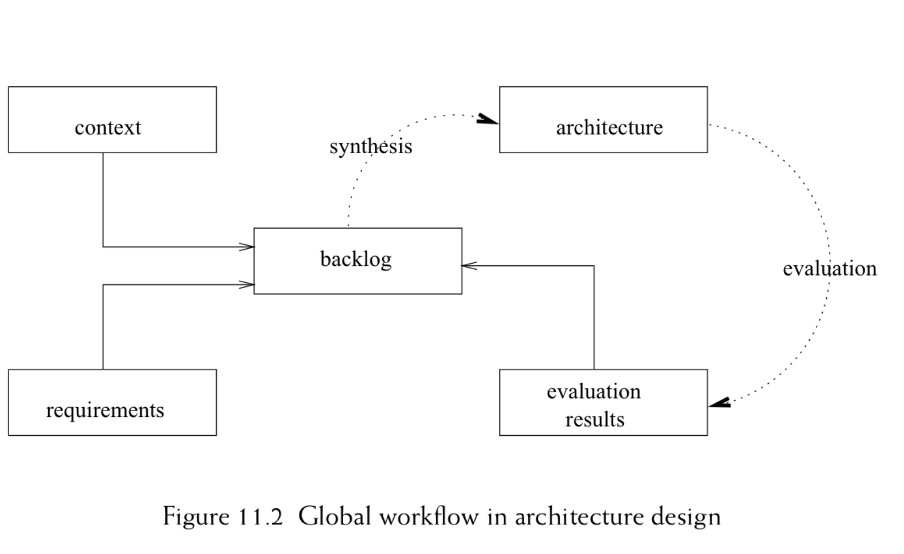
\includegraphics[scale = 0.75]{"Immagini/GeneralizedModel.png"}
\subsection{Decisioni di design} 
\subsection{Decision 1}
\begin{itemize} 
\item Issue 
\item Decision
\item Status 
\item Assumptions
\item Alternatives
\item Rationale
\item Implications
\item Notes
\end{itemize}
E' stato creato nei diagrammi UML diverse versioni dello stesso tipo di diagramma a seconda dello stakeholder
con cui ci si sta confrontando
TODO: AGGIUNGERE MODELLO CON COMPONENTI E CONNETTORI!!!

\subsection{Rappresentazione architettura con IEEE 1471} 
Le rappresentazioni più concrete dell'architettura dell'applicativo vengono descritte attraverso degli schemi UML. Questi possono essere categorizzati come delle View indirizzate a diversi Stakeholder e definite tramite diversi Viewpoint, come formalizzato dallo standard IEEE 1471.
\\In particolare, i Viewpoint utilizzati per definire le View sono stati scelti tra quelli proposti da Bass et al. (2003).
\subsubsection{Module View}
I Viewpoint nella categoria module costituiscono una rappresentazione statica del sistema. Per questo progetto la module view più importante è Class. 
\\Le view costruite seguendo le specifiche del viewpoint Class descrivono il sistema in termini delle relazioni di eredità degli elementi. Il class diagram UML del progetto mette a disposizione questa informazione, assieme ad altre precisazioni dovute alla natura object-oriented del linguaggio di programmazione. 
\\\textbf{Add image}
\subsubsection{Component and connector View}
Il tipo di viewpoint scelto in questa categoria è il process viewpoint. Questo definisce il sistema in termini di comunicazione e sincronizzazione di processi. 
\\Come tutti gli altri viewpoint in questa categoria, offre una descrizione dinamica del software e, nel caso particolare del process viewpoint, è particolarmente utile per valutare performance e availability del sistema. 
\\In termini di UML, questa informazione è disponibile principalmente tramite il Sequence diagram. Questo schema spiega come i diversi elementi (classi) del sistema comunicano tra di loro attraverso procedure calls \textbf{(di tipo sincrono e asincrono)}.
\subsubsection{Allocation View}
Questa categoria di viewpoint descrive la relazione tra il sistema e il mondo che lo circonda. Di conseguenza, può essere utilizzato per definire come viene assegnato hardware al software o come quest’ultimo viene mappato al file system. 
\\Per il progetto in questione, questo tipo di problematiche vengono gestite automaticamente dai framework utilizzati e quindi non sono competenza degli stakeholder che altrimenti ne farebbe uso, come i programmatori e i maintaner.
\\I viewpoint di tipo work assignment potrebbero essere utile per rappresentare graficamente la distribuzione del lavoro, ma in questo sprint vengono saltati per brevità. 

\section{Software Design}
I design pattern utilizzati per il progetto sono il factory e di conseguenza il simpleton, la classe user in questo caso occupa il ruolo di factory e si occupa di creare le classi stesse.
\\La classe User (presente nelle classi e nel diagramma delle classi) usa il design pattern Singleton che, in Dart, usa a sua volta una Factory per costruire l'istanza.

\section{Software Testing}
\subsubsection{IEEE928}
Questo tipo di documento si occupa di specificare e documentare come avviene la fase di testing
del progetto. Questo documento rappresenta anche il test plan. Siccome stiamo facendo un tipo di
sviluppo di software AGILE i test non vengono fatti alla fine ma vengono svolti in contemporanea allo
sviluppo delle classi.
\\Viene svolto un tipo di sviluppo di tipo TDD in cui si scrivono le classi dei test in 
contemporanea (se non prima) delle classi che servono per il sito. Le fasi del testing sono le 
seguenti:
\begin{itemize}
    \item Preparation of tests 
    \item Running the  tests
    \item Completion of testing
\end{itemize}

\subsubsection{Preparation of tests}
I test vengono fatti in contemporanea allo sviluppo delle classi, talvolta per alcune classi
sono stati fatti prima i test pensando poi alle classi che sarebbero state implementate successivamente.
I test per le classi in dart vengono scritti anche loro in linguaggio dart ed eseguiti tramite Junit.
\\Per quanto riguarda il testing di flutter si utilizza la funzione testWidgets che si importa 
dal pacchetto $flutter_test$ e permette di fare i test sulla web app.
\\Per garantire la CI (continuos integration) si utilizzerà Travis CI con i test che partiranno ad
ogni git e ogni 24 ore.
\\I test tenderanno ad essere il più possibile di tipo coverage in quanto si cercerà di coprire 
il più possibile i casi di test.
\\I test di Travis partono ogni 24 h sul main e ogni git su un branch specifico porta all'esecuzione 
del test in background su Travis. Ad ogni test viene fatta in automatico anche una build che permette
di vedere se ci sono eventuali errori di calligrafia all'interno del codice.
\\All'interno del progetto flutter vengono utilizzate 3 classi differenti che si occupano dello 
sviluppo del testing, essi sono:
\begin{itemize}
    \item $UnitTest.dart$: per fare unit testing
    \item $WidgetTest.dart$: per fare i test delle widget
\end{itemize}

\subsubsection{Running the tests}
Una volta fatte le classi ed eseguiti i test si procede in modo iterativo a modificare il codice
finchè i test non danno tutti risultati positivi

\subsubsection{Completion of testing}
I dati expected sono inventati e ad ogni iterazione si commentano i risultati per capire 
se va tutto bene e se c'è qualcosa che non quadra.
\subsection{Software Maintenance}
Siccome non sapevamo fin da principio come utilizzare Flutter e firebase abbiamo alternato momenti di forwading engeneering con momenti di reverese
engeneering in cui si è sistemata la documentazione in funzione del codice che è stato scritto (redocumentation).
\\Per quanto riguarda il refactoring sono stati utilizzati i tool che Visual code per eseguire il refactoring (come ad esempio 
la possibilità di wrappare le widget o cambiare a cascata il nome di una classe).
\\Una parte di refactoring è stato fatto utilizzando il comando dart analyze per rendersi conformi il più possibile agli standard di flutter 
\end{document}
